\documentclass[specialist,
               substylefile = ../spbu.rtx,
               subf,href,colorlinks=true, 10pt]{disser}

\usepackage[a4paper,
            mag=1000, includefoot,
            left=3cm, right=1.5cm, top=2cm, bottom=2cm, headsep=1cm, footskip=1cm]{geometry}
\usepackage[T2A]{fontenc}
\usepackage[utf8]{inputenc}
\usepackage[english,russian]{babel}

\let\bibfont\relax
\usepackage{biblatex}
\addbibresource{../biblio-u.bib}

\ifpdf\usepackage{epstopdf}\fi

% Точка с запятой в качестве разделителя между номерами цитирований
%\setcitestyle{semicolon}

% Использовать полужирное начертание для векторов
% \let\vec=\mathbf

% Включать подсекции в оглавление
\setcounter{tocdepth}{2}

\usepackage{graphicx}
\graphicspath{ {../media}, {.} }

\usepackage[intlimits]{amsmath}
\usepackage{amsfonts}
\usepackage{amssymb}
\usepackage{amsthm}

\usepackage{hyperref}
\newtheorem{theorem}{Теорема}
\newcommand{\ev}{\mathrm{E}}
\newcommand{\vfi}{\varphi}
\newcommand{\eps}{\varepsilon}
\newcommand{\prob}[1]{\mathrm{P}\left(#1\right)}
\newcommand{\R}{\ensuremath{\mathbb{R}}}
\newcommand{\Tau}{\ensuremath{\mathcal{T}}}
\newcommand{\GothB}{\mathfrak{B}}
\newcommand{\norm}[1]{\left\lVert#1\right\rVert}
\newcommand{\Vhat}{\hat{V}}
\newcommand{\vhat}{\hat{v}}
\newcommand{\maxset}[1]{\max\left\lbrace#1\right\rbrace}
\newcommand{\deltat}{\Delta t}
\DeclareMathOperator{\correlation}{cor}
\newcommand{\corr}[2]{\correlation\left(#1, #2\right)}
\DeclareMathOperator*{\argmax}{arg\,max}
\DeclareMathOperator*{\argmin}{arg\,min}
\DeclareMathOperator{\dd}{d}

% \usepackage[fixlanguage]{babelbib}
% \selectbiblanguage{russian}
% \setbtxfallbacklanguage{russian}


%----------------------------------------------------------------
\begin{document}

%
% Титульный лист на русском языке
%

% Название организации
\institution{%
    Санкт-Петербургский государственный университет \\
    Прикладная математика и информатика \\
    Статистическое моделирование
}

\title{Отчет о научно-исследовательской работе}

% Тема
\topic{\normalfont\scshape%
    Методы оценки Американского опциона}

% Автор
\author{Миллер Анастасия Александровна}

% Научный руководитель
\sa       {С.\,М.~Ермаков}
\sastatus {д.\,ф.-м.\,н., профессор}

% Город и год
\city{Санкт-Петербург}
\date{\number\year}

\begin{large}
\maketitle
\end{large}
\intro
В этом семестре моей задачей было наиболее полное сравнение двух методов оценки стоимости Американского опциона: по сетке и по дереву. Ниже даны краткие описания методов.
\section{Оценки по сетке и по дереву} % (fold)
\subsection{По сетке}\label{sub:mesh} % (fold)
Из \cite{Broadie2004,Kashtanov2015}.Из начального состояния $X_0$ для оценки опциона с $m$ моментами исполнения (состояние которого в $k$-й момент исполнения обозначается как $X_k$), равноотстоящими во времени от 0 до $T$, зададим сетку $X_n^i, n\in 1\mathbin{:}m, i \in 1\mathbin{:}b$, узлы которой --- реализации случайной величины с плотностью $p_{0, n}(X_0, \cdot)$ (маргинальные плотности; также рассматриваются средние плотности), а $p_{k, n}(x, y) = \prob{X_n = y \middle\vert X_k = x}$. Тогда определяется $\rho_{n, j}(x, y) = p_{n-1, n}(x, y) / p_{0, n}(X_0, y)$, сокращённые обозначения $\rho_{n, j}(i, j) = \rho_{n, j}(X_{n-1}^i, X_n^j)$ и оценка в каждом узле сетки
$$\hat Y_n(i) = \max\left\lbrace h_n(i), \frac{\sum_j \rho_{n+1}(i, j) \hat Y_{n+1}(j)}{\sum_j \rho_{n+1}(i, j)} \right\rbrace.$$

Тогда оценка справедливой стоимости опциона --- это $$\hat Y_0 = \max\left\lbrace h_0(X_0), \frac{\sum_j \rho_{1}(X_0, X_1^j) \hat Y_{1}(X_1^j)}{\sum_j \rho_{1}(X_0, X_1^j)} \right\rbrace.$$

% subsection по_сетке (end)

\subsection{По дереву} % (fold)
% \label{sub:по_дереву}

Из \cite{Broadie1997,Glasserman2004}. В аналогичных обозначениях оценка по дереву определяется через набор состояний $X_n^{j_1\cdots j_n}$, рекурсивно определяемых друг через друга как реализации случайной величины с плотностью $p_{n-1, n}(X_{n-1}^{j_1\cdots j_{n-1}})$. Тогда
$$\hat V_n^{j_1\cdots j_n} = \maxset{ h_n(X_n^{j_1\cdots j_n}), \frac{1}{b}\sum_{j=1}^b \hat V_{n+1}^{j_1\cdots j_n j}}$$
и оценка справедливой стоимости опциона -- это $$\hat V_0 = \maxset{ h_0(X_0), \frac{1}{b}\sum_{j=1}^b \hat V_{1}^{j}}.$$

\chapter{Теоретический анализ}
\section{Для $m = 1$} % (fold)
Для оценки по сетке $\rho_{1}(X_0, X_1^j) = p_{0, 1}(X_0, X_1^j) / p_{0, 1}(X_0, X_1^j) = 1$, а узлы $X_1^j$ порождены плотностью $p_{0, 1}(X_0, \cdot)$, т.е. 
$$\hat Y_0 = \maxset{ h_0(X_0), \frac{1}{b}\sum_j h_1(X_1^j) },$$
для оценки по дереву $$\Vhat_0 = \maxset{ h_0(X_0), \frac{1}{b} \sum_j h_1(X_1^j) },$$
то есть оценки совпадают по своей структуре.

\section{Для конечного числа состояний} % (fold)
Дискретизуем некоторым образом наше пространство состояний актива: пусть в момент $t_k$ актив может находиться только в некотором подмножестве состояний $\mathcal X_k = \left\lbrace x_{k}^i \right\rbrace_{i = 1}^{N_k}$ (дискретизация не обязана совпадать с сеткой, получающейся при использовании оценки по сетке, но все узлы из обоих методов для момента $t_k$ обязаны принадлежать $\mathcal X_k$).

Тогда оценку по дереву можно переписать как $$\Vhat_n^{j_1\cdots j_n} = \maxset{ h_n(X_n^{j_1\cdots j_n}), \sum_{j=1}^{N_{n+1}} w_n^{j_1\cdots j_n j}\hat V_{n+1}^{j_1\cdots j_n j}},$$
где $w_n^{j_1\cdots j_n j}$ --- эмпирическая оценка частоты выпадения $x_{n+1}^j \in \mathcal X_{n+1}$ как дочернего узла $X_n^{j_1 \cdots j_n}$. Эмпирическую оценку можно заменить точным значением, так как его можно посчитать для конечного числа состояний:
$$\Vhat_n^{j_1\cdots j_n} = \maxset{ h_n(X_n^{j_1\cdots j_n}), \sum_{j=1}^{N_{n+1}} p_{n, n+1}(X_n^{j_1\cdots j_n}, x_{n+1}^j) \hat V_{n+1}^{j_1\cdots j_n j}},$$
и здесь структура дерева уже вырождается, так как мы начинаем учитывать все возможные переходы, а не только $b$ случайных. Избавляясь от не несущих в такой постановке дополнительной информации символов, получаем
\begin{equation}
    \label{eq:discretized_tree}\Vhat_n^i = \maxset{ h_n(x_n^i), \sum_{j = 1}^{N_{n + 1}} p_{n, n+1}(x_n^i, x_{n+1}^j) \Vhat_{n+1}^j}.
\end{equation}А здесь уже видно, что \eqref{eq:discretized_tree} --- это оценка того же вида, что и предложенная в \cite{Broadie2004}, улучшением которой до конечной дисперсии и является оценка по сетке из раздела \ref{sub:mesh}.

\chapter{Численный анализ}

В статьях \cite{Broadie1997}, \cite{Broadie1997a} и \cite{Kashtanov2015} приведены результаты численных экспериментов с использованием описываемых методов. К сожалению, среди них нет ни одного примера, позволяющего сравнить оценки, полученные различными методами, для одного и того же набора параметров. Я реализовала оба метода (оценку по дереву --- в одном из предыдущих семестров, над оценкой по сетке я работала в этом семестре) в модели Блэка-Шоулса, чтобы сравнить получаемые ими оценки на однородных примерах.

\section{Детали реализации}

Согласно модели Блэка-Шоулса, состояние базового актива $X_t$ подчиняется геометрическому Броуновскому движению:
\begin{equation}\label{eq:black-scholes}
\dd X_t = X_t\left(\left(r - \delta\right)\dd t + \sigma \dd W_t\right),
\end{equation}
где $W_t$ -- стандартный винеровский случайный процесс, $r, \delta, \sigma$ -- параметры процесса. Далее будем обозначать $\mu = r - \delta$. Если базовый актив многомерный (несколько акций, возможно, коррелирующих между собой), то  $W_t = \left(w_t^{(1)}, \ldots, w_t^{{n}}\right)$. В таком случае добавляются параметры корреляции $\Sigma = \left\{\rho_{ij}\right\}_{i, j = 1}^n$:
$$\forall\: i, j \in 1 \mathbin : n \; \corr{w_t^{(i)}}{w_t^{(j)}} = \rho_{ij}.$$

Наивный (без методов уменьшения дисперсии) алгоритм оценки по дереву не вызывает особенных сложностей в реализации: генерация и обход дерева в глубину, в модели Блэка-Шоулса логнормально распределённые состояния базового актива генерируются по стандартной формуле, решающей уравнение \eqref{eq:black-scholes}:
\begin{equation*}
\forall j \in 1\mathbin{:}b \; X_{n+1}^{j_1\cdots j_n j} = X_{n}^{j_1\cdots j_n}e^{\left(\mu - \frac{\sigma^2}{2}\right)\deltat + \sigma \sqrt{\deltat} \eps_j}, \eps_j \sim \mathcal{N}\left(0, \Sigma\right).
\end{equation*}

Алгоритм оценки по сетке требует более аккуратного подхода: наивная реализация с подстановкой формул без упрощения является численно нестабильной. Как отмечается в \cite{Kashtanov2013}, для моделирования $X_n^j$ можно перейти к нормально распределённым случайным величинам $\eps_n^j$, связанным с $X_n^j$ следующим преобразованием: 
$$X_n^j = X_0 e^{\lambda n \deltat + \sigma \sqrt{n \deltat} \eps_n^j}.$$
Тогда выражение для переходной плотности
$$p_{k, n}\left(X_k^i, X_n^j\right) = \frac{1}{X_n^j\sqrt{2\pi\sigma^2\left(n-k\right)\deltat}}\exp\left( -\frac{\left(\ln X_n^j - \ln X_k^i - \left(\mu - \frac{\sigma^2}{2}\right)\left(n - k\right)\deltat \right)^2}{2\sigma^2 \left(n - k\right)\deltat} \right)$$
превращается в 
$$p_{k, n}\left(\eps_k^i, \eps_n^j\right) = \frac{1}{X_n^j \sqrt{2\pi\sigma^2 \left(n - k\right) \deltat}} \exp\left(-\frac{\left(\sqrt{n} \eps_n^j - \sqrt{k} \eps_k^i\right)^2}{2\left(n-k\right)}\right),$$
а веса $\rho_{n, j}(i, j)$ выглядят следующим образом:
$$\rho_{n, j}(i, j) = \sqrt{n}\exp\left( 
- \frac{1}{2}\left(\sqrt{n} \eps_n^j - \sqrt{n-1} \eps_{n-1}^i\right)^2
+ \frac{1}{2}\left(\eps_n^j                                   \right)^2\right).$$

\section{Численные результаты}

Текущие результаты вместе с референсными значениями представлены в табл.~\ref{tbl:mesh},~\ref{tbl:tree}, графическое представление -- на рис.~\ref{fig:mesh},~\ref{fig:tree}

\begin{table}[ht]
\caption{Оценка стоимости Американского опциона методом стохастической сетки (согласно \cite{Kashtanov2015})}
\center
	\begin{tabular}{crrrrr}
	$S_0$&$n$&истинное значение&$\hat Y_0$&$\mathrm{Var} \hat Y_0$\\\hline
	&10&&1.148&1.944\\
	70&100&0.121&0.908&0.103\\
	&1000&&0.871&0.009\\\hline
	&10&&8.392&23.37\\
	100&100&5.731&7.379&1.455\\
	&1000&&6.856&0.144\\\hline
	\end{tabular}
	% \label{fig:mesh_plot}
	\\\hfill
	\\\hfill
	\footnotesize{Параметры опциона: $r = 5\%, \delta = 10\%, \sigma = 20\%$. Начальная цена актива $S_0 = 100$, цена страйк $K = 100$, опцион выписан на $T=1$ год. Опцион имеет 4 момента исполнения: в $0, T/3, 2T/3$ и $T$.}
	\label{tbl:mesh}
\end{table}
\begin{figure}
\center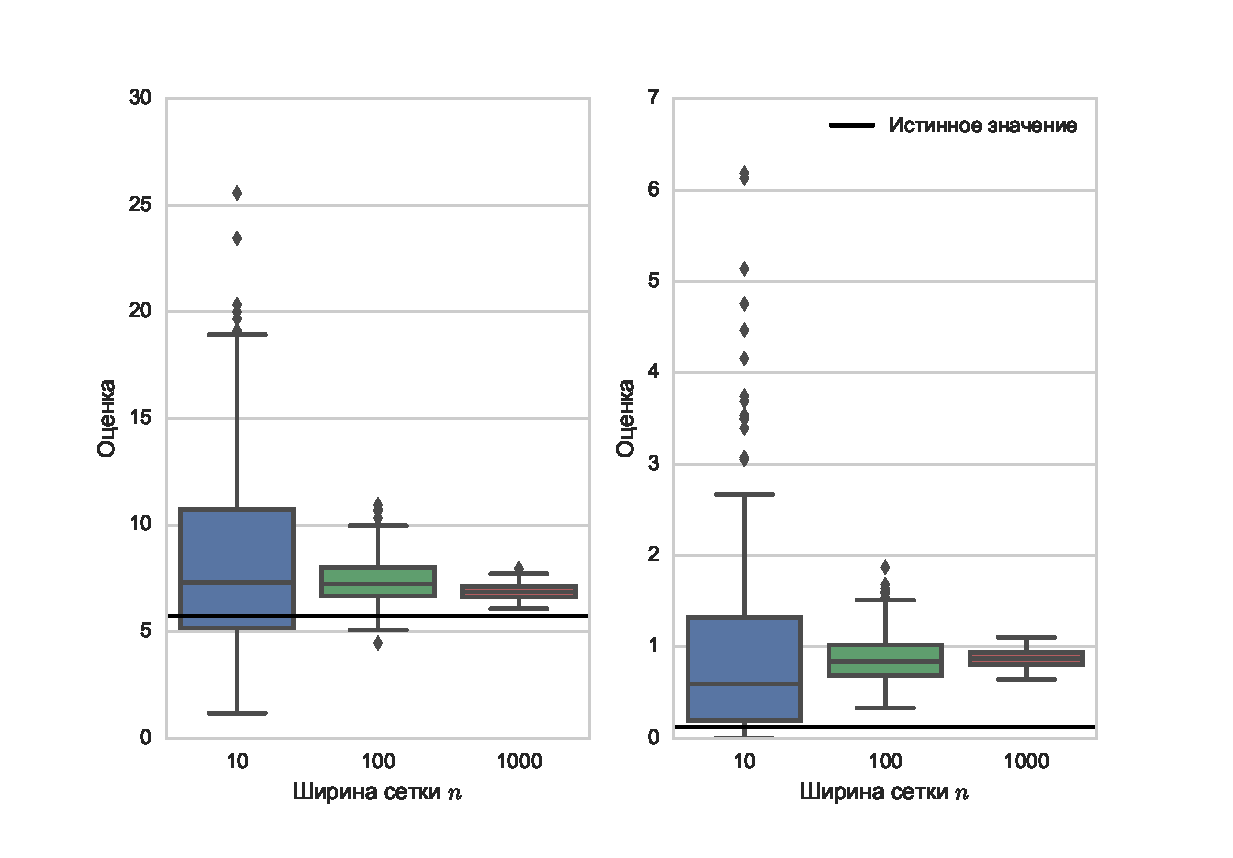
\includegraphics[width=\textwidth]{mesh_plot.eps}
	\caption{Оценка стоимости Американского опциона методом стохастической сетки (согласно \cite{Kashtanov2015})}
	% \label{fig:mesh_plot}
	\footnotesize{Параметры опциона: $r = 5\%, \delta = 10\%, \sigma = 20\%$. Начальная цена актива $S_0 = 100$, цена страйк $K = 100$, опцион выписан на $T=1$ год. Опцион имеет 4 момента исполнения: в $0, T/3, 2T/3$ и $T$.}
	\label{fig:mesh}
\end{figure}

% \begin{table}
% \center
% 	\begin{tabular}{c|rrrrr}
% 	$n$ & $S_0$ & $\hat Y_0$ & $\mathrm{Var} \hat Y_0$ & истинное значение \\ \hline
% 	10 & 70	& 0.689379&1.224001 & 0.121\\ 
% 	10 & 100 & 8.878406&18.439165 & 5.731\\ 
% 	100 & 70&0.992688&0.105836  & 0.121\\ 
% 	100 & 100 & 9.755667&2.072060 & 5.731\\
% 	1000 & 70 & 1.016055&0.013808 & 0.121\\
% 	1000 & 100 & 9.679787&0.187500 & 5.731\\
% 	\end{tabular}
% 	\caption{Оценки стоимости Американского опциона методом стохастической сетки}
% 	\label{tbl:mesh}
% \end{table}

\begin{table}[ht]
\center
	\caption{Оценка стоимости Американского опциона методом случайного дерева (согласно \cite{Broadie1997})}
	\begin{tabular}{c|rrrrr}
	$b$ & $S_0$ & $\hat V_0$ & $\mathrm{Var} \hat V_0$ & истинное значение \\ \hline
	10 & 100 & 5.859964 & 4.722421 & 5.731\\ 
	100 & 100 & 5.853083 & 0.344833 & 5.731\\
	200 & 100 & 5.661913 & 0.204637& 5.731\\
	300 & 100 & 5.777360 & 0.128013& 5.731\\
	\end{tabular}
	\\\hfill
	\\\hfill
	\footnotesize{Параметры опциона: $r = 5\%, \delta = 10\%, \sigma = 20\%$. Начальная цена актива $S_0 = 100$, цена страйк $K = 100$, опцион выписан на $T=1$ год. Опцион имеет 4 момента исполнения: в $0, T/3, 2T/3$ и $T$.}
	% \caption{Оценки стоимости Американского опциона методом случайного дерева}
	\label{tbl:tree}
\end{table}

\begin{figure}
\center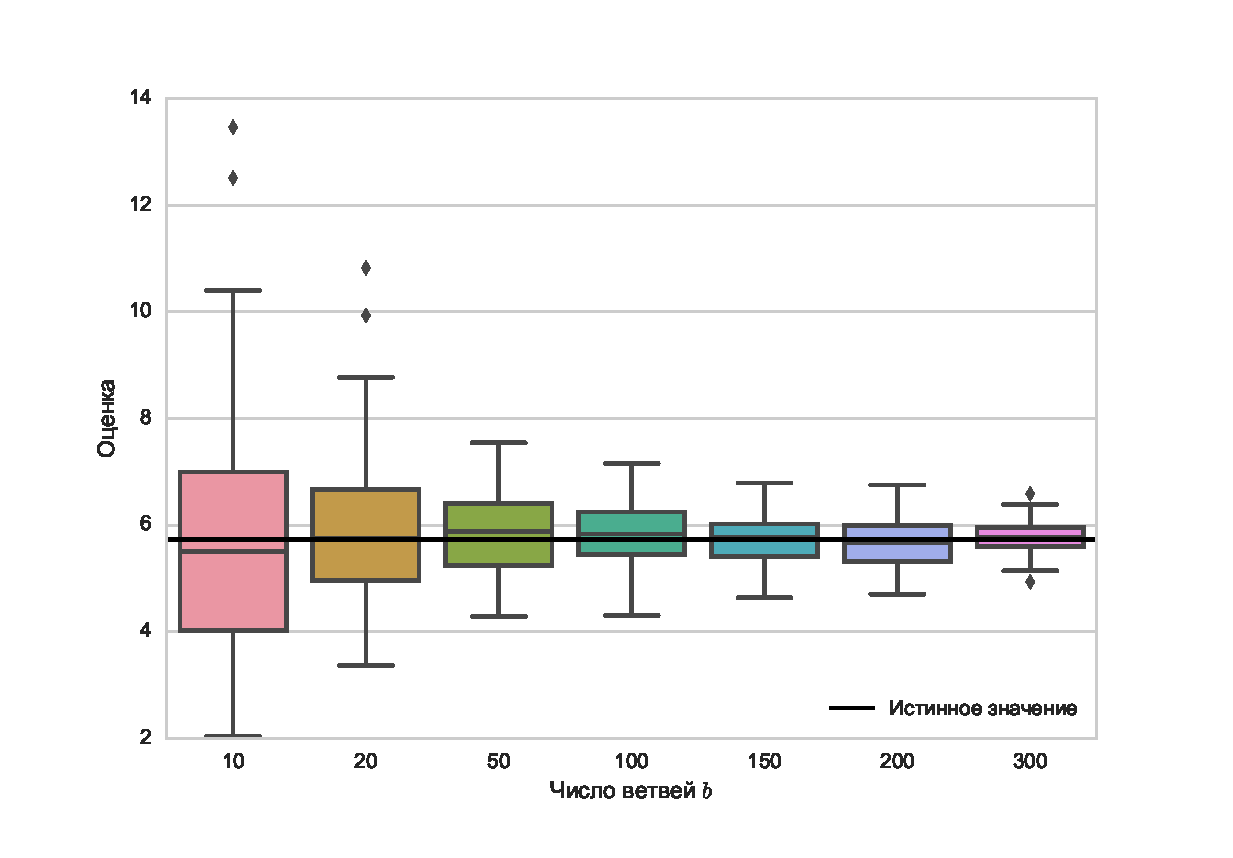
\includegraphics[width=0.7\textwidth]{tree_plot.eps}
	\caption{Оценка стоимости Американского опциона методом случайного дерева (согласно \cite{Broadie1997})}\label{fig:tree}
	\footnotesize{Параметры опциона: $r = 5\%, \delta = 10\%, \sigma = 20\%$. Начальная цена актива $S_0 = 100$, цена страйк $K = 100$, опцион выписан на $T=1$ год. Опцион имеет 4 момента исполнения: в $0, T/3, 2T/3$ и $T$.}
\end{figure}

% \begin{table}
% \center
% 	\begin{tabular}{c|rrrrr}
% 	$b$ & $S_0$ & $\hat V_0$ & $\mathrm{Var} \hat V_0$ & истинное значение \\ \hline
% 	10 & 100 & 5.859964 & 4.722421 & 5.731\\ 
% 	100 & 100 & 5.853083 & 0.344833 & 5.731\\
% 	200 & 100 & 5.661913 & 0.204637& 5.731\\
% 	300 & 100 & 5.777360 & 0.128013& 5.731\\
% 	\end{tabular}
% 	\caption{Оценки стоимости Американского опциона методом случайного дерева}
% 	\label{tbl:tree}
% \end{table}


% \chapter{Существующие исследования}

% Также был проведён небольшой анализ источников и ссылок для того, чтобы найти сравнимые результаты численных экспериментов.

% \paragraph{\cite{Broadie2008}} Представлены результаты для одномерного случая, сравнимые с \cite{Broadie1997}, и для многомерного, сравнимые с \cite{Broadie2004}.


% \bibliographystyle{ugost2008}
% \bibliography{../biblio-u}


\printbibliography

\end{document}

